%%%%%%%%%%%%%%%%%%%%%%%%%%%%%%%%%%%%%%%%%%%%%%%%%%%%%%%%%%%%%%%%%%%%%%%%%%%%%%%%%%%%%%%%%%%%%%%%%%%%%%
% Plantilla básica de Latex en Español.
%
% Autor: Andrés Herrera Poyatos (https://github.com/andreshp)
%
% Es una plantilla básica para redactar documentos. Utiliza el paquete fancyhdr para darle un
% estilo moderno pero serio.
%
% La plantilla se encuentra adaptada al español.
%
%%%%%%%%%%%%%%%%%%%%%%%%%%%%%%%%%%%%%%%%%%%%%%%%%%%%%%%%%%%%%%%%%%%%%%%%%%%%%%%%%%%%%%%%%%%%%%%%%%%%%%

%-----------------------------------------------------------------------------------------------------
%	INCLUSIÓN DE PAQUETES BÁSICOS
%-----------------------------------------------------------------------------------------------------

\documentclass{article}

\usepackage{lipsum}                     % Texto dummy. Quitar en el documento final.

%-----------------------------------------------------------------------------------------------------
%	SELECCIÓN DEL LENGUAJE
%-----------------------------------------------------------------------------------------------------

% Paquetes para adaptar Látex al Español:
\usepackage[spanish,es-noquoting, es-tabla, es-lcroman]{babel} % Cambia
\usepackage[utf8]{inputenc}                                    % Permite los acentos.
\selectlanguage{spanish}                                       % Selecciono como lenguaje el Español.

%-----------------------------------------------------------------------------------------------------
%	SELECCIÓN DE LA FUENTE
%-----------------------------------------------------------------------------------------------------

% Fuente utilizada.
\usepackage{courier}                    % Fuente Courier.
\usepackage{microtype}                  % Mejora la letra final de cara al lector.

%-----------------------------------------------------------------------------------------------------
%	ESTILO DE PÁGINA
%-----------------------------------------------------------------------------------------------------

% Paquetes para el diseño de página:
\usepackage{fancyhdr}               % Utilizado para hacer títulos propios.
\usepackage{lastpage}               % Referencia a la última página. Utilizado para el pie de página.
\usepackage{extramarks}             % Marcas extras. Utilizado en pie de página y cabecera.
\usepackage[parfill]{parskip}       % Crea una nueva línea entre párrafos.
\usepackage{geometry}               % Asigna la "geometría" de las páginas.

% Se elige el estilo fancy y márgenes de 3 centímetros.
\pagestyle{fancy}
\geometry{left=3cm,right=3cm,top=3cm,bottom=3cm,headheight=1cm,headsep=0.5cm} % Márgenes y cabecera.
% Se limpia la cabecera y el pie de página para poder rehacerlos luego.
\fancyhf{}

% Espacios en el documento:
\linespread{1.1}                        % Espacio entre líneas.
\setlength\parindent{0pt}               % Selecciona la indentación para cada inicio de párrafo.
\usepackage{hyperref}
\usepackage{algorithm}
\usepackage{algpseudocode}
\usepackage{graphicx}
% Cabecera del documento. Se ajusta la línea de la cabecera.
\renewcommand\headrule{
	\begin{minipage}{1\textwidth}
	    \hrule width \hsize
	\end{minipage}
}

% Texto de la cabecera:
\lhead{\docauthor}                          % Parte izquierda.
\chead{}                                    % Centro.
\rhead{\subject \ - \doctitle}              % Parte derecha.

% Pie de página del documento. Se ajusta la línea del pie de página.
\renewcommand\footrule{
\begin{minipage}{1\textwidth}
    \hrule width \hsize
\end{minipage}\par
}

\lfoot{}                                                 % Parte izquierda.
\cfoot{}                                                 % Centro.
\rfoot{Página\ \thepage\ de\ \protect\pageref{LastPage}} % Parte derecha.


%-----------------------------------------------------------------------------------------------------
%	PORTADA
%-----------------------------------------------------------------------------------------------------

% Elija uno de los siguientes formatos.
% No olvide incluir los archivos .sty asociados en el directorio del documento.
\usepackage{title1}
%\usepackage{title2}

%-----------------------------------------------------------------------------------------------------
%	TÍTULO, AUTOR Y OTROS DATOS DEL DOCUMENTO
%-----------------------------------------------------------------------------------------------------

% Título del documento.
\newcommand{\doctitle}{Algoritmos genéticos y Differential Evolution en Sentiment Analysis}
% Subtítulo.
 \newcommand{\docsubtitle}{}
% Fecha.
\newcommand{\docdate}{1 \ de \ Enero \ de \ 2015}
% Asignatura.
 \newcommand{\subject}{}
% Autor.
\newcommand{\docauthor}{Nuria Rodríguez Barroso}
\newcommand{\docaddress}{Universidad de Granada}
\newcommand{\docemail}{rbnuria@correo.ugr.es}

%-----------------------------------------------------------------------------------------------------
%	RESUMEN
%-----------------------------------------------------------------------------------------------------

% Resumen del documento. Va en la portada.
% Puedes también dejarlo vacío, en cuyo caso no aparece en la portada.
%\newcommand{\docabstract}{}
\newcommand{\docabstract}{Aplicación de algoritmos genéticos y Differential evolution para la optimización del comportamiento de herramientas de extracción de polaridad}

\begin{document}

\maketitle

%-----------------------------------------------------------------------------------------------------
%	ÍNDICE
%-----------------------------------------------------------------------------------------------------

% Profundidad del Índice:
%\setcounter{tocdepth}{1}

\newpage
\tableofcontents
\newpage

%-----------------------------------------------------------------------------------------------------
%	SECCIÓN 1
%-----------------------------------------------------------------------------------------------------

\section{Introducción}

	\subsection{Contexto}
	En los últimos años, la minería de datos ha obtenido tal relevancia en nuestra sociedad que cada vez se considera más indispensable a la hora de la toma de decisiones en una corporación. Estamos rodeados de todo tipo de datos: afinidades, ubicaciones, opiniones, información personal, etc.
	
	Una corporación o empresa, como sabemos, ofrece un producto al cliente con el fin de satisfacerlo y además lucrarse. Sería de gran interés para esta empresa conocer cuál es la opinión del cliente sobre el producto, cuáles son las mejoras que él añadiría y cuáles son los defectos que él eliminaría. 
	
	Actualmente, obtener una opinión de un cliente sobre tu producto es mucho más fácil que pasar una encuesta, gracias a la Web 2.0. Basta con analizar las redes sociales, que están en continuo crecimiento, o analizar otras fuentes de opiniones como pueden ser TripAdvisor, Google, Amazon,etc. Pero, ¿cómo analizaríamos estas opiniones, sobre todo cuando tu producto es comprado y valorado por miles de personas? Efectivamente, hacerlo contratando personal que valore estos comentarios resultaría inviable, tanto por el tiempo que llevaría como por los recursos económicos que habría que invertir.
	
	Sentiment Analysis pretende dar una solución a este problema.  Se trata de un campo de la minería de datos que, según \cite{tanetal}, se centra en la extracción de información útil a partir de textos. Este tema cada vez está obteniendo mayor popularidad en el ámbito de la computación. Como vemos en la figura \ref{fig:relevancia} obtenida a partir de Google Trends, durante los últimos años, Sentiment Analysis ha ido ganado popularidad en las búsquedas, un claro reflejo de que se trata de un campo cada vez más importante y útil.
\begin{figure}[h]
	\centering
	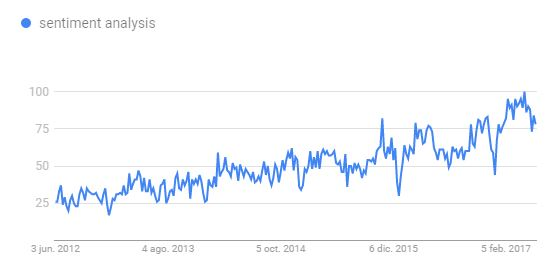
\includegraphics[width=0.7\linewidth]{relevancia}
	\caption{Relevancia del Sentiment Analysis según las búsquedas realizadas en Google}
	\label{fig:relevancia}
\end{figure}
\newpage
\subsection{Sentiment Analysis y descripción del problema}
Sentiment Analysis podría definirse como un problema de clasificación (ver \ref{fig:clasificationscheme}) en el que el objetivo es identificar el sentimiento que un texto transmite. Se trata de un problema cuya principal dificultad recae en el tratamiento de información difusa, en la que además de factores más objetivos como la ortografía, existen también otros factores subjetivos tales como la ironía o el sarcasmo, a veces siendo estos difíciles de entender incluso por los seres humanos.

Para obtener esta clasificación, existen varias alternativas:
\begin{itemize}
	\item \textbf{Aproximación por Aprendizaje Automático.} El problema se trata con técnicas de aprendizaje automático tales como Support Vector Machine o técnicas basadas en árboles. Pueden ser problemas supervisados o no supervisados. En los primeros el principal problema es que debemos tener un gran conjunto de comentarios ya etiquetados con el fin de aprender a partir de estos comentarios etiquetados. En los segundos, nuestro sentimiento se extrae a partir de funciones heurísticas u otras reglas predefinidas.
	\item \textbf{Aproximación por técnicas basadas en diccionarios.} Estas técnicas se basan en diccionarios elaborados manualmente donde cada palabra tiene una intensidad de sentimiento asociada. Alternativamente a las técnicas basadas en diccionarios tenemos las técnicas basadas en corpus, donde se tienen en cuenta distintos patrones sintácticos tales como palabras que expresan conectividad o por ejemplo contradicción.
	\item  \textbf{Aproximación por herramientas de Procesamiento del Lenguaje Natural (NLP).} Estas herramientas emplean técnicas computacionales (Aprendizaje automático, inteligenia artificial, inferencia estadística...) unidas a técnicas basadas en lingüística para darnos la polaridad de un texto. Se puede definir también como un software que integra alguna de las 2 técnicas nombradas anteriormente (o ambas) y que ha sido desarrollado con fines comerciales o de investigación, facilitando al usuario el proceso de Sentiment Analysis (sin que este tenga que desarrollar su propio modelo o su propio diccionario).
\end{itemize}

\begin{figure}
	\centering
	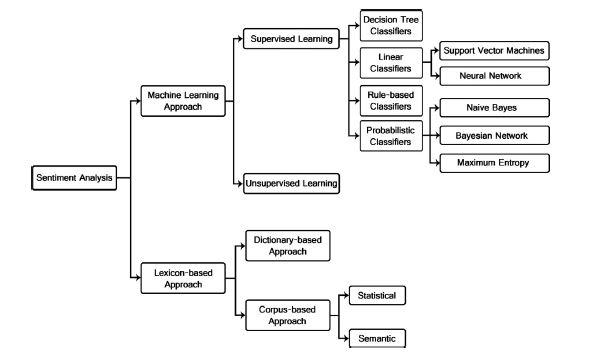
\includegraphics[width=0.7\linewidth]{clasificationScheme}
	\caption{Esquema del problema de Sentiment Analysis}
	\label{fig:clasificationscheme}
\end{figure}

\newpage
\textbf{Nuestro problema}

Nuestro problema consiste en la optimización del comportamiento de 7 herramientas de Procesamiento de Lenguaje Natural (NLP) o herramientas de extracción de polaridad con respecto al etiquetado experto de un total de 20 datasets de comentarios y la comparación de los resultados con otra alternativa que es la agregación de estas herramientas con una ponderación equitativa, la cual denomiremos 'Solución Trivial'. Esta optimización del comportamiento se realizará mediante la asignación de pesos a las herramientas, siendo estos pesos buscados mediante algoritmos genéticos primero y posteriormente técnicas de Differential evolution. Estos pesos representan la importancia de cada máquina siendo 1 el 100\% y 0 un 0\%. Las herramientas que hemos usado son las siguientes:
\begin{enumerate}
	\item \textbf{Azure Text Analytics. } Se trata de una API de Microsoft Azure con fines comerciales pero que aun así ofrece una versión de prueba gratuita con hasta 5000 llamadas de la función para obtener el sentimiento. Al tratarse de una herramienta comercial, no se conoce cómo funcionan exactamente, aunque en su documentación se aclara que está diseñada con el fin de que funcione bien en textos cortos.
	\item \textbf{Bing. } Esta herramienta contiene un diccionario con términos
	clasificados previamente como positivos, neutros y negativos. De esta
	manera, compara las palabras a clasificar con el diccionario. Esta
	herramienta está basada en diccionarios. 
	\item \textbf{coreNLP. } Es una herramienta de código abierto de la \textit{Stanford University} que ha sido entrenada empleando redes neuronales sobre comentarios de películas.
	\item \textbf{MeaningCloud}. Esta herramienta aplica diferentes técnicas de
	preprocesado y posteriormente realiza una clasificación que puede ser
	binaria (positivo o negativo) o multiclase (muy positivo, positivo, neutro,
	negativo, muy negativo). Este método utiliza Machine Learning
	para analizar texto que proviene de diferentes fuentes. Actúa evaluando
	las relaciones que existen en una frase y el texto entero y termina
	devolviendo el valor de la polaridad.
	\item \textbf{SentiStrength. }Esta herramienta estima la fuerza de positividad
	o negatividad que existe en una frase aplicando un método con dos
	maneras de medir a la vez, ya que el ser humano puede llegar a expresar
	dos sentimientos opuestos al mismo tiempo. Utiliza Machine Learning
	y métodos basados en diccionarios. Ha sido entrenada sobre comentarios de Twitter.
	\item \textbf{Syuzhet. } Este método se basa en diccionarios implementado por \textit{Nebraska Literary Lab}.
	\item \textbf{Vader. } Es un método basado en diccionaros y funciones heurísticas y reglas que está ajustado para funcionar bien en sentimientos expresados en los medios de comunicación.
\end{enumerate}

Partiremos de las intensidades que cada herramienta nos devuelve para cada comentario y nuestro objetivo es que la combinación lineal de las intensidades de cada herramienta ponderadas con el peso de la solución minimice el error cuadrático, aunque los resultados se mostrarán según el error de clasificación para ser interpretado más fácilmente.

El problema también tiene algunas restricciones, como el hecho de que los pesos del vector solución tienen que sumar 1. Esto lo solucionamos, primero generando las soluciones iniciales de forma que se mantenga la restricción y posteriormente en los genéticos realizando un cruce aritmético y en el resto de casos normalizando según los mínimo y máximo del vector solución (normalización min-max).


Los experimentos han sido realizados haciendo una 5-fold cross validation, que consiste en crear 5 particiones de los datos y para cada experimento aprendemos los pesos con 4 de estas particiones y validamos con la otra.
\subsection{Preparación de los datos}
Los datos son obtenidos a partir de los resultados de la ejecución de las distintas herramientas sobre las bases de datos. Cada característica será la intensidad del sentimiento que cada herramienta nos devuelve con respecto a cada comentario.

Como cada herramienta nos devuelve su resultado en un dominio distinto, normalizaremos con el fin de que todas las herramientas tengan la misma importancia en la búsqueda de los pesos. Normalizaremos en el intervalo [0,1], siendo 0 el valor de intensidad más negativo para un comentario y 1 el más positivo.

Para los primeros experimentos trabajaremos con un dataset formado por todos los comentarios (los de las 20 bases de datos) juntos.
\section{Algoritmos genéticos}
Para este estudio vamos a considerar dos tipos de algoritmos genéticos, que surgen de la combinación del operador de cruce aritmético con 2 esquemas de evolución diferentes:
\begin{itemize}
	\item \textbf{Esquema generacional con elitismo: } Por un lado, vamos a considerar un esquema de evolución generacional, esto es, se seleccionará una generación de padres del mismo tamaño de la población genética que serán posteriormente cruzados y mutados (algunos de ellos). Para mantener el elitismo, nos aseguraremos de que la mejor solución de la población anterior siga apareciendo en la nueva generación. Para ello, si esto no ocurre sustituiremos la peor solución generada en la nueva población por la mejor de la anterior.
	\item \textbf{Esquema estacionario: } Por otro lado, consideraremos un esquema de evolución estacionario, donde seleccionaremos dos padres que serán posteriormente cruzados y mutados (no siempre, ya lo veremos). Los cromosomas resultado del cruce y mutación de los padres generados, sustituirán a los dos cromosomas más débiles de la población anterior (peor función objetivo) en caso de no ser ellos mismos. 
\end{itemize}

En cuanto al operador de cruce, como ya se ha comentado, usamos un \textbf{Operador CA}, u operador de cruce aritmético, que cada dos cromosomas padres, genera un cromosoma hijo fruto de la media aritmética componente a componente de ambos padres. Esto es, considerando los padres anteriores, el hijo sería de la forma:

\[
c_{hijo} = ( \frac{c_{11} + c_{21}}{2}, ..., \frac{c_{1n} + c_{2n}}{2})
\]

Como este operador genera cada dos padres un único hijo, para generar el mismo número de hijos que con el operador BLX, habrá que utilizar el doble de padres. Esta consideración la veremos con detalle más adelante.

En cuanto a la probabilidad de cruce y mutación para cada uno de los algoritmos genéticos vamos a utilizar, en primer lugar, las probabilidades utilizadas en la práctica 1, que son: 0.7 de probabilidad de cruce (en el generacional) y un 0.001 de probabilidad de mutación por gen producido.

Los resultados obtenidos aplicando como criterio de parada 500000 evaluaciones de la función objetivo han sido:
\begin{table}[H]
	\begin{center}
		\scalebox{1.2}{
			\begin{tabular}{|l|l|l|l|}
				\hline
				Algoritmo & Acierto clasificación & Tiempo & Acierto solución trivial\\ \hline
				AGG-CA  & 54.33\% & 177.7627 &  55.76\%\\ \hline
				AGE-CA & 53.96  \% & 177.6286 & 55.76\%\\ \hline
		\end{tabular}}
		\caption{Algoritmos genéticos.}
		\label{tabla:a1}
	\end{center}
\end{table}

Como podemos observar las soluciones obtenidas no mejoran en media a los resultados obtenidos con la solución trivial. Es por ello que nos planteamos realizar ciertas mejoras sobre estos algoritmos.
\subsection{Mejoras planteadas}
\subsubsection{Truncamiento de pesos}
Debido al operador de cruce que utilizamos, un peso nunca valdrá 0 debido a que se hace una media aritmética. Para solucionar esto vamos a cambiar el operador de cruce truncando los pesos a 0 cuando sean menores que 0.1 y a 1 cuando sean mayores de 0.9. Con el mismo objetivo realizaremos esta mejora sobre también las soluciones iniciales generadas aleatoriamente para que no ocurra lo mismo sobre las soluciones que nunca se cruzan.

Los resultados obtenidos aplicando como criterio de parada 500000 evaluaciones de la función objetivo han sido:
\begin{table}[H]
	\begin{center}
		\scalebox{1}{
			\begin{tabular}{|l|l|l|l|}
				\hline
				Algoritmo & Acierto clasificación & Tiempo & Acierto solución trivial\\ \hline
				AGG-CA  & 54.33\% & 177.7627 &  55.76\%\\ \hline
				AGG-CA Truncado & 53.96\% & 195.4605  &  55.76\%\\ \hline
				AGE-CA & 53.96  \% & 177.6286 & 55.76\%\\ \hline
				AGE-CA Truncado & 53.52\% & 174.3407 & 55.76\%\\ \hline
		\end{tabular}}
		\caption{Algoritmos genéticos con truncamiento de pesos}
		\label{tabla:a2}
	\end{center}
\end{table}

Como podemos observar con esta mejora seguimos sin mejorar la solución trivial, además de que las mejoras son poco significativas.
\subsubsection{Reducción de la probabilidad de mutación}
Basándonos en la idea del enfriamiento simulado, aquella que dice que en las primeras etapas del algoritmo se favorezca a la exploración y en las últimas a la explotación, nos planteamos dar una probabilidad más alta de mutación a las soluciones en las primeras etapas e ir reduciéndolas proporcionalmente. Ahora la probabilidad de mutación será 0.5 por cada gen y se irá reduciendo en un 10\% en cada etapa.

Los resultados obtenidos aplicando como criterio de parada 500000 evaluaciones de la función objetivo han sido:

\begin{table}[H]
	\begin{center}
		\scalebox{1}{
			\begin{tabular}{|l|l|l|l|}
				\hline
				Algoritmo & Acierto clasificación & Tiempo & Acierto solución trivial\\ \hline
				AGG-CA  & 54.33\% & 177.7627 &  55.76\%\\ \hline
				AGG-CA con enfriamiento de probabilidad & 55.56\% &  191.5620  &  55.76\%\\ \hline
				AGE-CA & 53.96  \% & 177.6286 & 55.76\%\\ \hline
				AGE-CA con enfriamiento de probabilidad & 54.58\% & 201.6321 & 55.76\%\\ \hline
		\end{tabular}}
		\caption{Algoritmos genéticos con enfriamiento de probabilidad de mutación}
		\label{tabla:a3}
	\end{center}
\end{table}

Combinando ambas modificaciones obtenemos los siguientes resultados:
\begin{table}[H]
	\begin{center}
		\scalebox{1}{
			\begin{tabular}{|l|l|l|l|}
				\hline
				Algoritmo & Acierto clasificación & Tiempo & Acierto solución trivial\\ \hline
				AGG-CA  & 54.33\% & 177.7627 &  55.76\%\\ \hline
				AGG-CA con ambas mejoras & 55.85\% &  188.7995  &  55.76\%\\ \hline
				AGE-CA & 53.96  \% & 177.6286 & 55.76\%\\ \hline
				AGE-CA con ambas mejoras & 53.90\% & 193.4081 & 55.76\%\\ \hline
		\end{tabular}}
		\caption{Algoritmos genéticos con enfriamiento de probabilidad de mutación}
		\label{tabla:a3}
	\end{center}
\end{table}
\subsubsection{Algoritmos meméticos}
Consiste en introducir una búsqueda local a determinados individuos de la generación cada ciertas etapas. Consideraremos 3 algoritmos meméticos, que se diferencian en los individuos afectados por la búsqueda local, pues en todos ellos se aplica cada 10 generaciones:

\begin{itemize}
	\item \textbf{AM (10, 1.0).} Consiste en aplicar cada 10 generaciones la búsqueda local a todos los individuos.
	\item \textbf{AM (10, 0.1).} Consiste en aplicar cada 10 generaciones la búsqueda local al 10\% de los individuos elegidos aleatoriamente.
	\item \textbf{AM (10, 0.1 MEJ).} Consiste en aplicar cada 10 generaciones la búsqueda local al mejor 10\% mejor de la población.
\end{itemize}

Para realizar los tres algoritmos meméticos vamos a considerar solo el algoritmo genético generacional, pues es el que mejores resultados ha proporcionado. Estas son las soluciones obtenidas con los meméticos:
\begin{table}[H]
	\begin{center}
		\scalebox{1}{
			\begin{tabular}{|l|l|l|l|}
				\hline
				Algoritmo & Acierto clasificación & Tiempo & Acierto solución trivial\\ \hline
				AGG-CA  & 53.70\% & 195.0211 &  55.76\%\\ \hline
				AM (10, 1.0) & 55.38\% & 180.92 & 55.76\%\\ \hline
				AM (10, 0.1) &  55.74\% & 185.54 & 55.76\%\\ \hline
				AM (10, 0.1 MEJ) & 55.74\% & 234.5 & 55.67\%\\ \hline
		\end{tabular}}
		\caption{Algoritmos meméticos}
		\label{tabla:a4}
	\end{center}
\end{table}


\section{Differential Evolution}
La evolución diferencial es un modelo evolutivo que enfatiza la mutación. Para ello utilizaremos un operador de cruce posterior a la mutación de los individuos. Partiremos de una población inicial de individuos totalmente aleatorios. Iremos produciendo hijos utilizando tres operadores que describiremos a continuación. Una vez generado el hijo, este competirá con su padre para ver cuál pertenece a la generación.

\begin{itemize}
	\item \textbf{DE/Rand/1: } El vector hijo se obtendrá mediante la siguiente fórmula
	\[
	V_{i,G} = X_{r1,G} + F (X_{r2,G} - X_{r3,G})
	\]
	donde los índices r1 ,r2 y r3 de cada individuo $i$ en cada generación $G$ serán escogidos aleatoriamente de forma mutuamente excluyente (incluyendo al vector i-ésimo).
	
	\item \textbf{DE/Current-to-best/1 :} En este caso, el vector mutación se obtiene a partir de la siguiente fórmula:
	
	\[
	V_{i,G} = X_{i,G} + F(X_{best,G} - X_{i,G}) - F(X_{r1,G} - X_{r2,G})
	\]
	
	Donde, análogamente al operador anterior, los índices $r1$ y $r2$ serán escogidos de forma aleatoria de forma mutuamente excluyente (incluyendo la posición $i$), mientras que $X_{best,G}$ denota el mejor individuo de la población $G$.
\end{itemize}

Como podemos observar, ambos operadores están basados en distancias con una cierta probabilidad. En el caso del primero, acercamos la solución en $p1$ a los otros dos padres, obteniendo así una combinación de estos tres padres en la componente $j$ y, en total, obteniendo el hijo mutado como una combinación de varios padres de la generación anterior. En el segundo caso, lo que hacemos es acercar el padre actual a la mejor solución y luego acercarlo a la combinación de los dos padres. 

Cuando nos referimos a que el cruce se realizará con cierta probabilidad, es que vamos a utilizar una recombinación binomial, esto es, el operador solo se aplicará si al obtener un número aleatorio entre (0,1) se encuentra por debajo de un cierto parámetro $CR$ previamente fijado.

La principal diferencia entre ambos operadores es que el primero fomenta la exploración, dado que realiza mutaciones más fuertes y totalmente aleatorias, mientras que el segundo fomenta la explotación, explotando la mejor solución hasta el momento generada acercando todos los hijos generados hacia esta solución.

El reemplazamiento en ambos algoritmos evolutivos será \textit{one-to-one}. Esto es, cada hijo generado competirá con su padre para sustituirle en la generación.

\begin{itemize}
	\item \textbf{ED/best/1.}  El operador de cruce no mueve la solución actual en la dirección del a mejor, si no que iguala a la mejor, y desplaza componente a componente los valores en función de dos soluciones de la población elegidas de forma aleatoria.
	
	Seguiría el siguiente esquema:
	
	\[
	V_{i,G} = X_{best,G} + F (X_{r1,G} - X_{r2,G})
	\]
	
	Por lo que el método explotará aún más la mejor solución hasta el momento ($X_{best,G}$ representa la mejor solución de la generación G).
\end{itemize}

Es fácil darse cuenta de que estos cruces producen soluciones no válidas para nuestro problema concreto. Para ello tras aplicar cada una de estas operaciones normalizaremos las soluciones en [0,1] de forma que la suma de la solución sea 1.

Los resultados con criterio de parada de 500000 evaluaciones de la función objetivo son los siguientes:
\begin{table}[H]
	\begin{center}
		\scalebox{1}{
			\begin{tabular}{|l|l|l|l|}
				\hline
				Algoritmo & Acierto clasificación & Tiempo & Acierto solución trivial\\ \hline
				DE/Rand  & 55.72\% & 192.0525 &  55.76\%\\ \hline
				DE/Current-to-best & 55.38\% & 180.92 & 55.76\%\\ \hline
				DE/Best/1 &  55.71\% & 190.6599 & 55.76\%\\ \hline
		\end{tabular}}
		\caption{Algoritmos meméticos}
		\label{tabla:a5}
	\end{center}
\end{table}

\section{Considerando diferentes corpus}
Dado que los resultados obtenidos por todos los métodos implementados (incluyendo mejoras) no son los esperados, nos planteamos si el problema reside en la base de datos. Como cada una de las máquinas consideradas ha sido entrenada sobre un tipo determinado de comentarios o han sido diseñadas para tipos de comentarios concretos, se obtienen resultados muy dispersos debido a que nuestro dataset inicial contiene comentarios desde tweets cogidos aleatoriamente hasta comentarios sobre noticias de la BBC. Por ello, vamos a probar los algoritmos implementados hasta ahora (los genéticos con las dos modificaciones) en algunos de los corpus por separado, para ver si así obtenemos resultados mejores. Si nuestra hipótesis se cumple, veremos que la solución obtenida en cada uno de los corpus dará más peso a diferentes máquinas.

Vamos a probar sobre las bases de datos:
\begin{itemize}
	\item \textbf{Pang movie (Movie Reviews).}
	\item \textbf{Aisopos ntua (Tweets Random).}
	\item \textbf{Sentistrength BBC (BBC news comments). }
	\item \textbf{Sentistrength YouTube (YouTube comments). }
	\item \textbf{Vader Amazon (Amazon product reviews). } 
\end{itemize}


\begin{table}[H]
	\begin{center}
		\scalebox{0.9} {
			\begin{tabular}{|l|l|l|l|l|l|l|l|l|l|l|}
				\hline
				& \multicolumn{2}{|c|}{Aisopos ntua} & \multicolumn{2}{|c|}{Pang movie} & \multicolumn{2}{|c|}{Sentistrength BBC}\\ \hline
				& Porcentaje acierto &Tiempo & Porcentaje acierto & Tiempo & Porcentaje acierto & Tiempo\\ \hline
				Trivial& 59.60\%& - & 50.60\% &  -& 49.60\% & -\\ \hline
				AGG-CA& 67.40\%& 1.9149 &64.04\%& 29.7155 & 63.80\%& 3.2296\\ \hline
				AGE-CA& 64.80\%& 1.9521 & 64.01\% & 29.8232 & 62.20\% &3.2819\\ \hline
				AM(10,1)& 68.00\%& 1.4341 &  64.25\% & 30.1023 & 62.50\%& 2.8962\\ \hline
				AM(10,0.1)& 68.00\%& 1.5179 &64.28\% & 30.1842 & 64.60\%& 2.9668\\ \hline
				AM(10,0.1mej)& 67.60\%& 1.4811 &64.24\% & 29.8356  & 60.40\%& 2.9061\\ \hline
				DE/Rand& 67.80\%& 1.7716 & 64.22\% & 29.4543  & 64.30\%&3.0238\\ \hline
				DE/Current-to-best& 67.60\%&  1.7402 & 64.23\% & 29.9380 & 63.20\%& 2.9881\\ \hline
				DE/Best/1& 67.80\%& 1.7096 &  64.24\%& 29.1250& 64.20\%& 3.0015\\ \hline
			\end{tabular}
		}\caption{Comparativo de los algoritmos en los diferentes corpus.}
		\label{tabla:corpus1}
	\end{center}
\end{table}

\begin{table}[H]
	\begin{center}
		\scalebox{1}{
			\begin{tabular}{|l|l|l|l|l|}
				\hline
				& \multicolumn{2}{|c|}{Sentistrength Youtube} & \multicolumn{2}{|c|}{Vader Amazon}\\ \hline
				& Porcentaje acierto & Tiempo & Porcentaje acierto & Tiempo\\ \hline
				Trivial&62.52\% & - & 48.27\%& -\\ \hline
				AGG-CA& 63.02\%& 9.4789 & 47.87\%& 10.5734\\ \hline
				AGE-CA& 61.46\%& 9.5385 & 47.11\%& 10.6590\\ \hline
				AM(10,1)& 62.93\%& 9.3697 & 46.79\% & 10.4552\\ \hline
				AM(10,0.1)& 62.87\%& 9.5427 & 47.73\% & 10.5505\\ \hline
				AM(10,0.1mej)& 62.70\%& 9.3301 & 46.98\% & 10.7551\\ \hline
				DE/Rand& 63.08\%& 9.4708 & 47.79\%& 10.6834\\ \hline
				DE/Current-to-best& 63.08\%&  9.4031 & 47.79\%& 10.8188\\ \hline
				DE/Best/1& 63.08\%& 9.3941 & 47.79\% & 10.8360 \\ \hline
			\end{tabular}
		}\caption{Comparativo de los algoritmos en los diferentes corpus.}
		\label{tabla:corpus2}
	\end{center}
\end{table}

Como vemos nuestros métodos mejoran la solución trivial en casi todos los corpus, a excepción de Vader Amazon (quizás por la complejidad y diversidad de los comentarios). De hecho, en este DataSet se comportan mejor algunas de las máquinas por separado:
\begin{itemize}
	\item Azure: 54.61\%
	\item bing: 51.24\%
	\item coreNLP: 54.37\%
	\item MeaningCloud: 54.8\%
	\item SentiStength: 21.39\%
	\item Syuzhet: 58.03\%
	\item Vader: 46.33\%
\end{itemize}
Creemos que este fracaso se debe a la complejidad de la base de datos, pues Amazon contiene gran diversidad de productos y con ello de público y opiniones.

Sin embargo, en algunos DataSets se produce mucha mejora con respecto a la solución trivial. Esto ocurre en aquellos DataSets que están formados por tipos de comentarios sobre los que han entrenado las máquinas.

Por ejemplo, en el DataSet \textit{Aisopos ntua} se llega a conseguir una mejora de casi el 19\% respecto de la solución trivial. Si consideramos algunas de las soluciones que han conseguido mejores resultados en alguna partición obtenemos:

\begin{itemize}
	\item AGG-CA: (0.3788 , 0.0000 , 0.0510 , 0.1098 , 0.2993 , 0.0000 , 0.1611) con un 75\% de acierto.
	\item AGE-CA: (0.3646  , 0.0000 , 0.1182 , 0.0000 , 0.5172 , 0.0000 , 0.0000) con un 78\% de acierto.
	\item AM(10,1): (0.3818  , 0.0000 , 0.0657 , 0.1123 , 0.3252 , 0.0000 , 0.1151) con un 76\% de acierto.
	\item AM(10,0.1): (0.3707 , 0.0000 , 0.0939 , 0.1108 , 0.3044 , 0.0000 , 0.1203) con un 77\% de acierto. 
	\item AM(10,0.1mej): (0.3786 , 0.0000 , 0.0417  , 0.1450 , 0.3109 , 0.0000 , 0.1238) con un 75\% de acierto. 
	\item DE/Rand: (0.3916 , 0.0000 , 0.0431 , 0.1173 , 0.3217 , 0.0000 , 0.1263) con un 77\% de acierto. 
	\item DE/Current-to-best: (0.3914, 0.0000 , 0.0432 , 0.1174 , 0.3217 , 0.0000 , 0.1262) con un 76\% de acierto. 
	\item DE/Best: (0.3916, 0.0000 , 0.0432 , 0.1172 , 0.3218 , 0.0000 , 0.1262) con un 77\% de acierto.
\end{itemize}

Como podemos observar, las máquinas con mayor peso son en todas las soluciones la primera (Azure) y la quinta (SentiStrength). Esto puede deberse a que SentiStrength sabemos que ha sido entrenada con comentarios de Twitter y la primera, según su propia documentación, ha sido diseñada para funcionar bien en comentarios de corto tamaño. Por ello, estas máquinas son las que obtienen mejores resultados y una combinación en la que predominen estas máquinas nos lleva a resultados mejores. Por ejemplo, en los dos primeros algoritmos meméticos obtenemos una tasa de acierto media de 68\%, mientras que el mejor resultado obtenido por una de estas máquinas es 63.2\% por Azure y el obtenido por la solución trivial es de 59.6\%.

Lo mismo ocurre con Pang movie, en el que la máquina que predomina (obteniendo un peso de más de 0.5 en todas las soluciones óptimas generadas) es coreNLP, la cual ha sido entrenada sobre comentarios de películas. En este caso, obtenemos con casi todos los algoritmos implementados una tasa de acierto parecida de sobre el 14\% de mejora sobre la solución trivial.

Algo diferente ocurre con el DataSet sentistrength\_BBC, en el que obtenemos también mejoras considerables con respecto a la solución trivial aunque ninguna de las máquinas ha sido entrenada sobre comentarios de este tipo. El comportamiento de las distintas herramientas sobre este corpus es:
\begin{itemize}
	\item \textbf{Azure: } 31.1\%
	\item \textbf{Bing: } 53.8\%
	\item \textbf{coreNLP: }63.9\%
	\item \textbf{MeaningCluod: } 44.7\%
	\item \textbf{SentiStrength: } 46.4\%
	\item \textbf{Syuzhet: }46.4\%
	\item \textbf{Vader: } 46.9\%
\end{itemize}

Mientras que la tasa de acierto con la solución trivial ha sido del 49.6\% y la tasa de acierto media del mejor algoritmo ha sido del 64.6\%. Las soluciones con una tasa de acierto de este rango se componen de la combinación lineal de las máquinas Bing, CoreNLP y MeaningCloud.

A continuación observamos en unas gráficas la importancia de las máquinas para cada uno de los corpus considerados (representamos la mejor solución obtenida en alguna partición):
\begin{figure}[H]
	\centering
	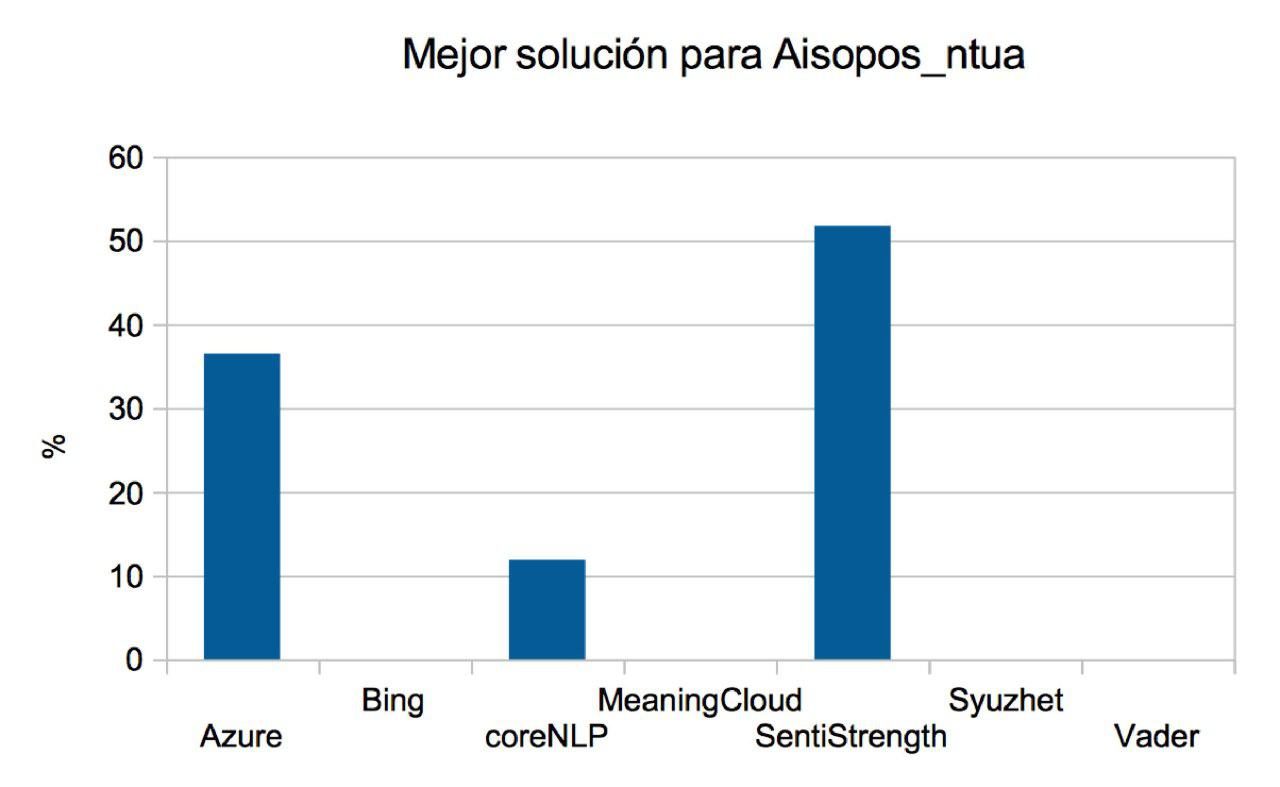
\includegraphics[width=0.7\linewidth]{aisopos_ntua}
	\caption{Pesos de las máquinas para aisopos\_ntua}
	\label{fig:aisoposntua}
\end{figure}

\begin{figure} [H]
	\centering
	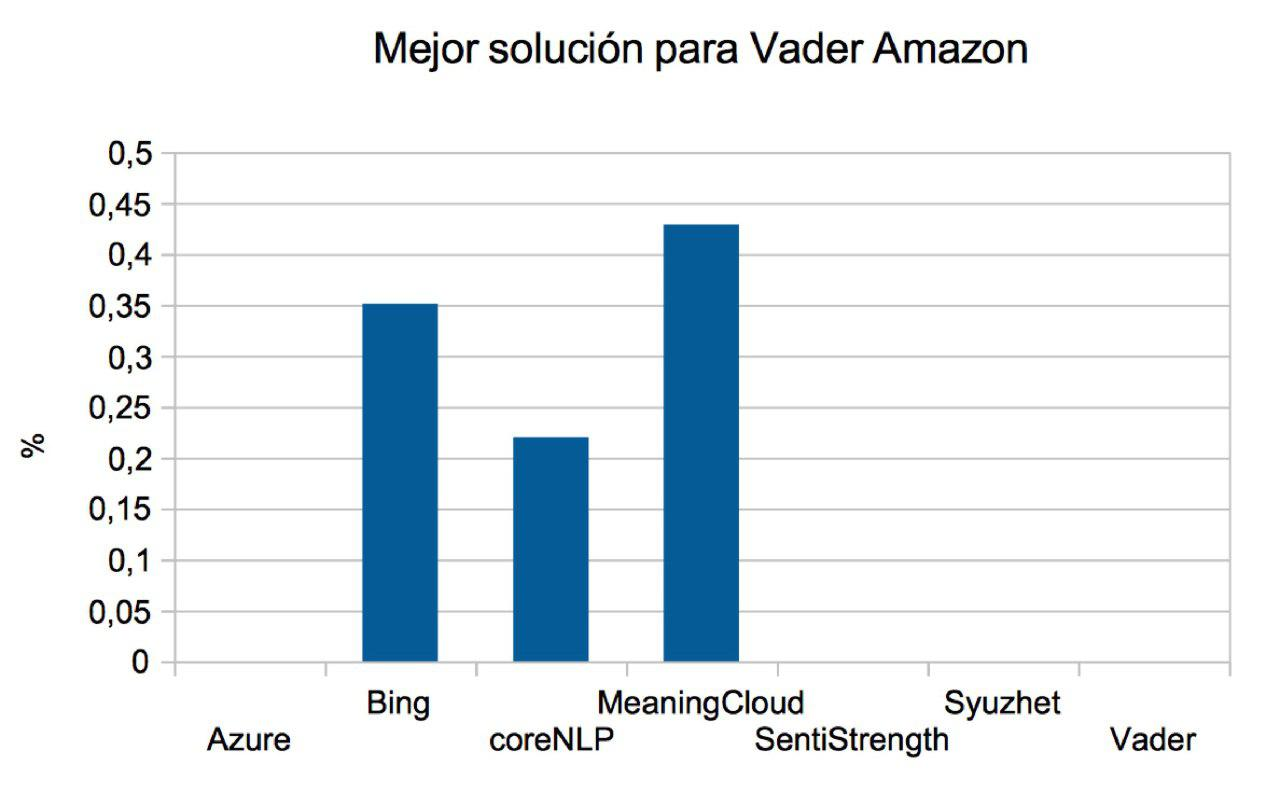
\includegraphics[width=0.7\linewidth]{amazon}
	\caption{Pesos de las máquinas para vader\_amazon}
	\label{fig:amazon}
\end{figure}

\begin{figure} [H]
	\centering
	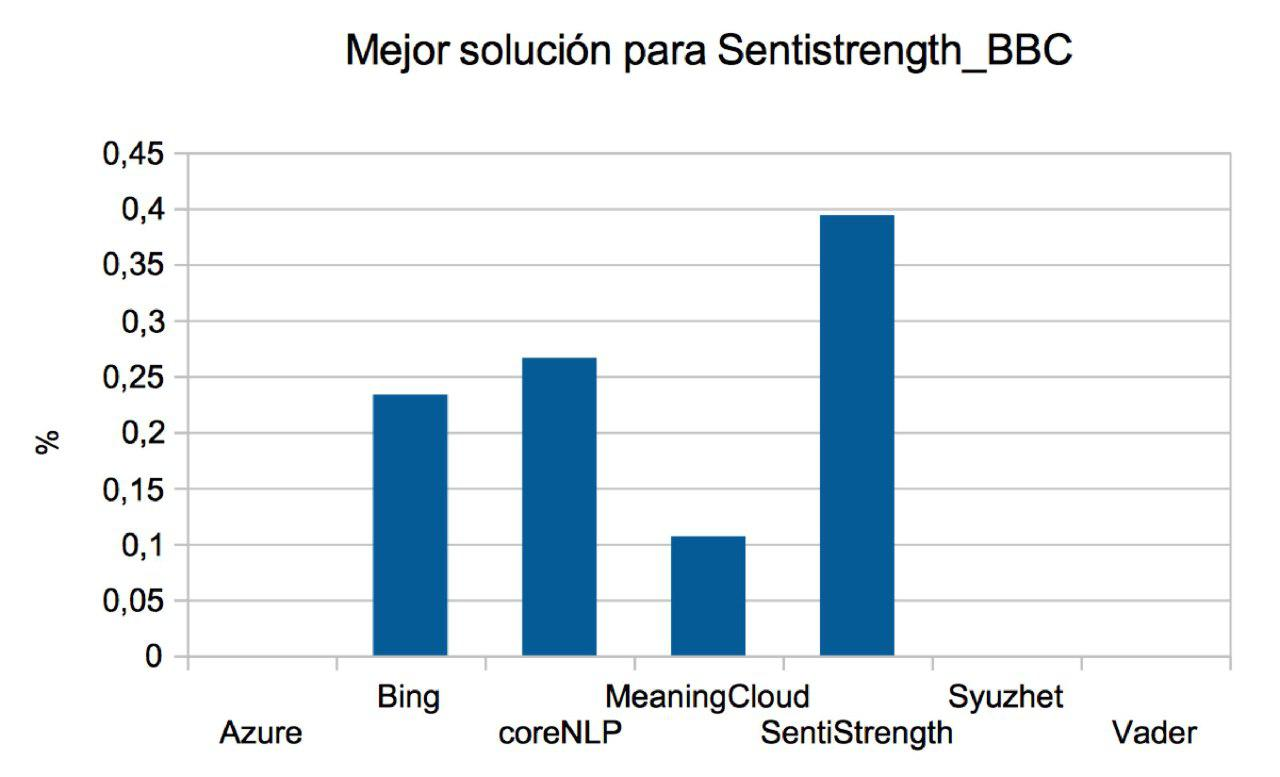
\includegraphics[width=0.7\linewidth]{bbc}
	\caption{Pesos de las máquinas para sentistrength\_bbc}
	\label{fig:bbc}
\end{figure}

\begin{figure} [H]
	\centering
	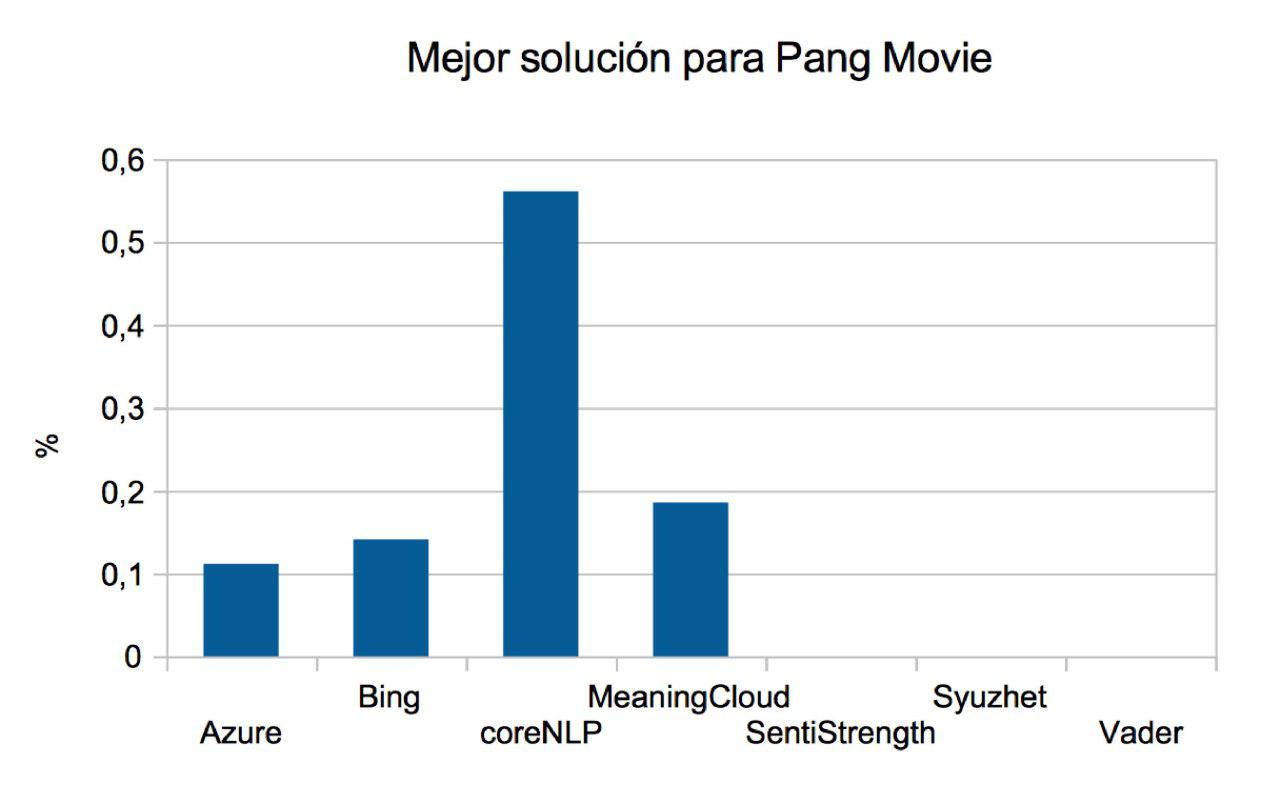
\includegraphics[width=0.7\linewidth]{pang_movie}
	\caption{Pesos de las máquinas para pang\_movie}
	\label{fig:pangmovie}
\end{figure}

\begin{figure} [H]
	\centering
	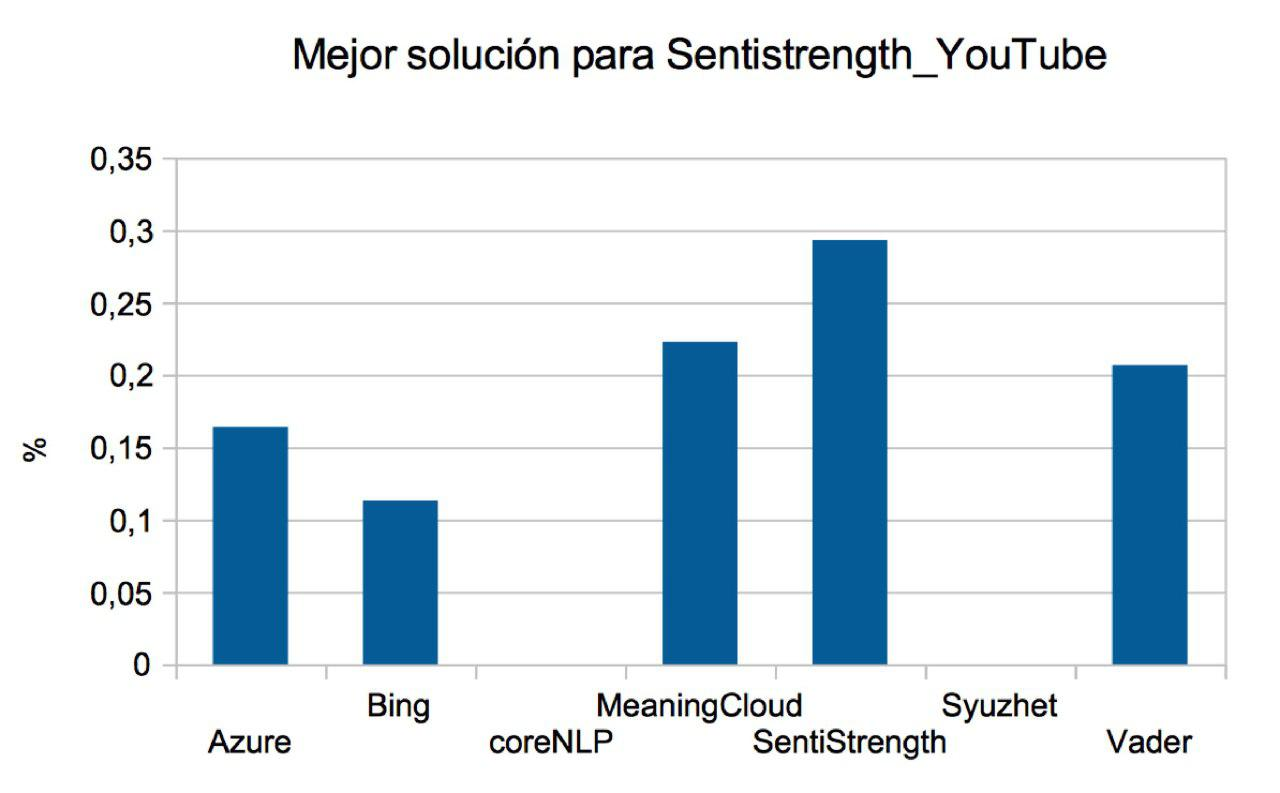
\includegraphics[width=0.7\linewidth]{youtube}
	\caption{Pesos de las máquinas para sentistrength\_youtube}
	\label{fig:youtube}
\end{figure}

A parte de lo ya comentado anteriormente sobre las soluciones obtenidas en cada corpus, simplemente resaltar la diversidad de ``mejores soluciones'' que se han obtenido dependiendo del problema, donde confirmamos que el problema de la primera aplicación de los algoritmos a la base de datos completa era la diversidad de tipos de comentarios, por lo que no hemos podido encontrar una combinación de estas máquinas que obtenga mayor tasa de acierto.

\section{Comparación entre los algoritmos implementados.}

	En esta sección vamos a estudiar la eficacia de los algoritmos implementados, aunque echando un vistazo rápido a las tablas generadas, podemos concluir rápidamente que no vamos a encontrar uno que sea mejor que otro de forma general, si no que dependerá del conjunto de trabajo. 
	
	En cuanto a los algoritmos genéticos, el algoritmo genético generacional ha obtenido siempre mejores resultados que el estacionario, llegando a superar hasta en un 3\% los resultados obtenidos por este segundo. Esto se debe a que el generacional favorece la exploración de soluciones y esto es imprescindible en este tipo de problema. 
	
	Vamos a estudiar la convergencia de ambos algoritmos genéticos durante las primeras 50 iteraciones en el DataSet Aisopos\_ntua (estudiamos los algoritmos genéticos con las mejoras dos implementadas), observamos los resultados en las Figuras \ref{fig:aggca} y \ref{fig:ageca}.
	
	En estas gráficas se ve claramente la importancia de la exploración con respecto a la explotación de soluciones. En cada generación del algoritmo genético generacional se producen más hijos, por lo cual, hay mayor diversidad en la búsqueda de soluciones, obteniendo soluciones mejores en menos tiempo (observamos la gran bajada que hay en las primeras iteraciones del método), aunque a partir de entonces el método no mejora mucho (de hecho no se llega a encontrar más mejora en el resto de iteraciones del método). Esto se puede deber a la disminución progresiva de la probabilidad de mutación por gen.
	
	 Por otro lado, el genético estacionario, al producir solo un hijo por generación es más lento en la búsqueda de soluciones. Observamos que sigue disminuyendo aún donde hemos dejado de imprimir las soluciones, sin embargo, ha conseguido en estas 50 iteraciones una solución peor que la que había conseguido ya el generacional en las 10 primeras. Así, podemos concluir que por regla general, el algoritmo AGG-CA obtendrá mejores resultados que el AGE-CA considerando el mismo número de iteraciones.
	
	\begin{figure}[H]
		\centering
		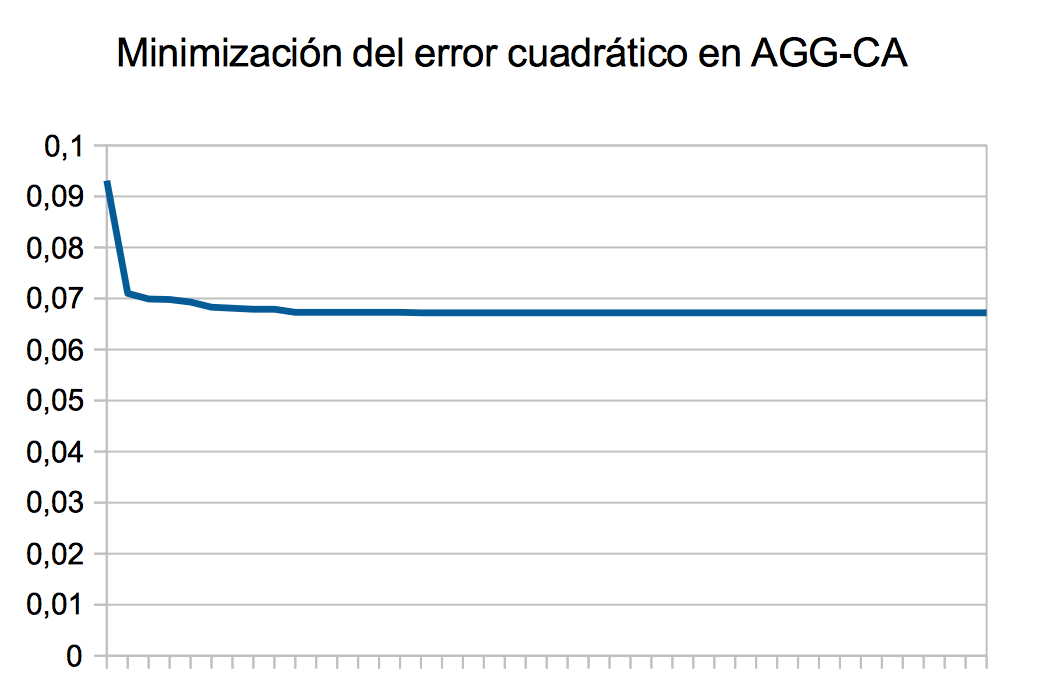
\includegraphics[width=0.7\linewidth]{aggca}
		\caption{Convergencia soluciones AGG-CA}
		\label{fig:aggca}
	\end{figure}

	\begin{figure}[H]
	\centering
	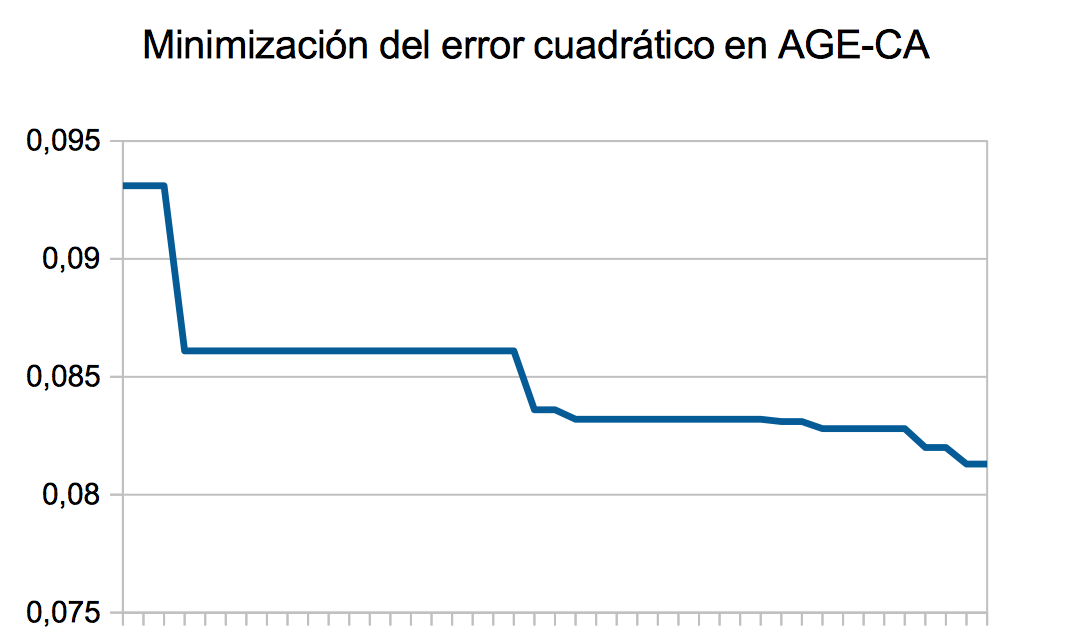
\includegraphics[width=0.7\linewidth]{ageca}
	\caption{Convergencia soluciones AGE-CA}
	\label{fig:ageca}
\end{figure}

	Ahora, si nos planteamos la importancia de las dos mejoras incluidas en los algoritmos genéticos básicos implementados, veamos cómo se comporta el algoritmo AGG-CA básico en las 50 primeras iteraciones sobre el mismo DataSet en Figura \ref{fig:aggcano}. 
	
	
	\begin{figure}[H]
		\centering
		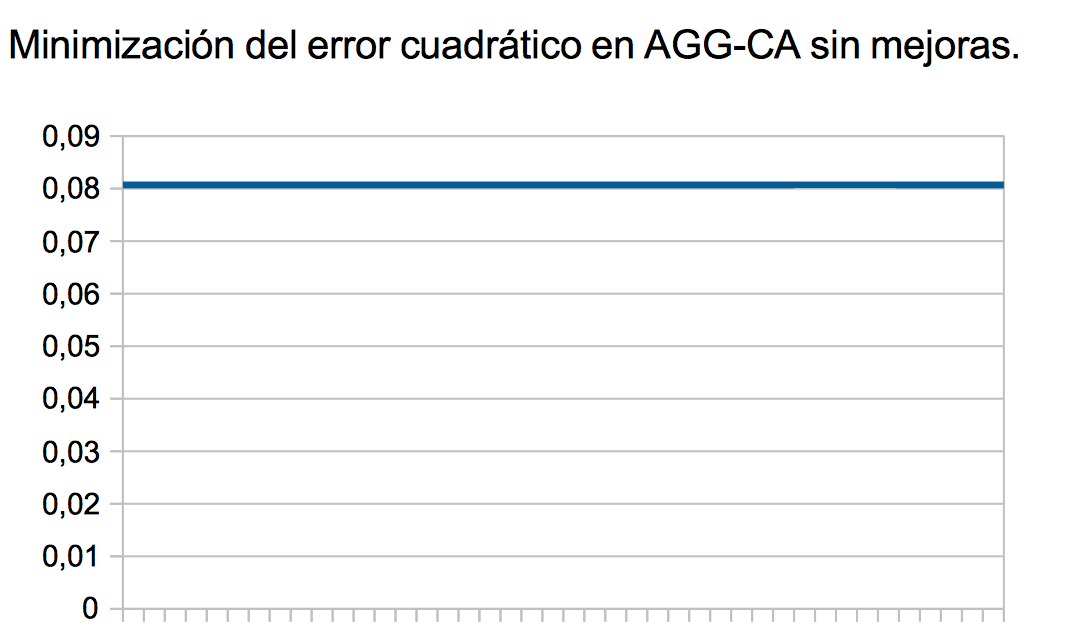
\includegraphics[width=0.7\linewidth]{aggca-nomejora}
		\caption{Convergencia soluciones AGG-CA sin mejora.}
		\label{fig:aggcano}
	\end{figure}

	Como podemos observar, la mejor solución obtenida en estas primeras 50 iteraciones no mejora. Esto se debe a que, ignorando las mejoras realizadas se complica la exploración de soluciones, dado que la mutación es mucho menor desde un principio y el cruce es menos brusco al no aplicar el truncamiento. 
	
	En cuanto a los meméticos implementados, la diferencia por regla general es poca. La diferencia entre estos algoritmos los individuos de la generación a los cuales se les aplica la búsqueda local. En el caso del primer memético, dado que se le aplica a todos, te aseguras no despreciar soluciones que con una búsqueda local pudieran dar soluciones buenas, a costa de utilizar muchas evaluaciones de la función objetivo para ello. En los otros dos sin embargo, se seleccionan ciertos individuos de la generación a los que aplicar la búsqueda local. En el primer caso de estos, se aplica aleatoriamente mientras que en el segundo a los mejores. Podríamos pensar que aplicarlo a los mejores tendría que dar mejores resultados siempre, sin embargo, soluciones que por sí solas produzcan un mayor error cuadrático pueden producir mejores soluciones al aplicar la búsqueda local, así, el primero de estos ha obtenido en ocasiones mejores resultados que el segundo.
	
	Por todo lo comentado, los tres meméticos tienen ventajas y desventajas y se comportan de forma parecida en los problemas considerados.
	
	Para terminar con este apartado, estudiamos los algoritmos diferenciales implementados.  En este caso, la similitud de resultados es incluso mayor aunque por regla general el que peor resultado ha obtenido ha sido el DE/Current-to-best. 
	
	Esto se debe a que el primero enfatiza la exploración de soluciones y el último la explotación, acercando siempre la solución hacia la mejor generada hasta el momento. El segundo de estos intenta enfatizar en explotación pero en menos medida. Por esto, se queda a medio camino entre ambas estrategias de búsqueda de soluciones obteniendo, de forma general, peores resultados.
	
	Para finalizar esta sección, vamos a estudiar el comportamiento de las soluciones generadas en un algoritmo de Differential Evolution (Rand). 
	
	\begin{figure}[H]
		\centering
		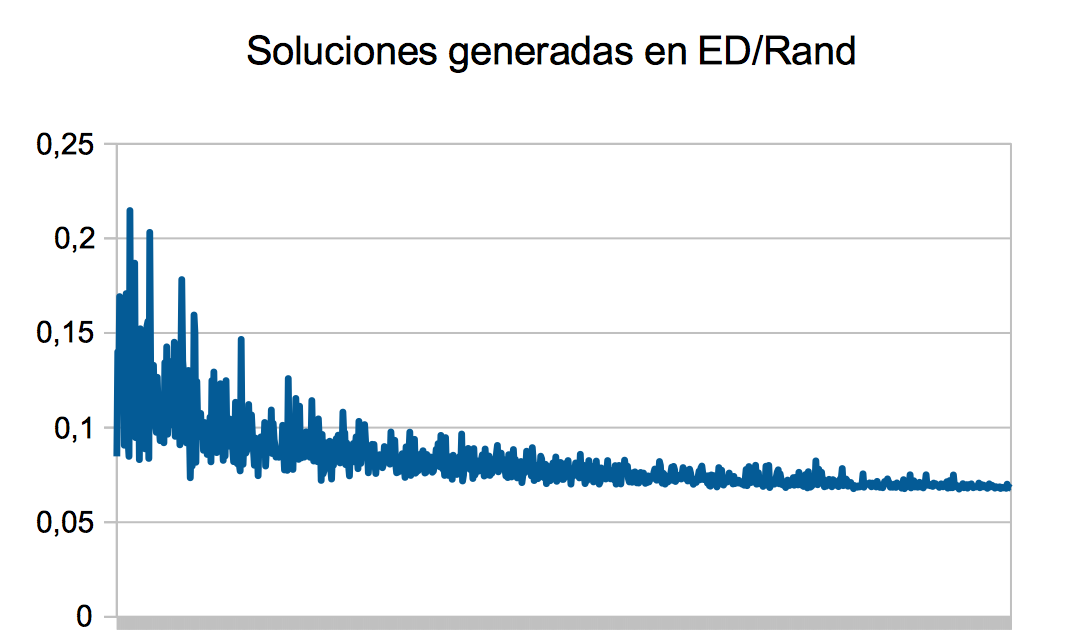
\includegraphics[width=0.7\linewidth]{rand}
		\caption{Soluciones generadas.}
		\label{fig:rand}
	\end{figure}
	

	Podemos observar en la Figura \ref{fig:rand} como se van generando soluciones de forma muy aleatoria (gran exploración) y va convergiendo poco a poco a la solución final obtenida.
	
	

\section{Comentarios finales.}
	

%-----------------------------------------------------------------------------------------------------
%	SECCIÓN 2
%-----------------------------------------------------------------------------------------------------}
\begin{thebibliography}{99}
\bibitem[Tan et al., 1999]{tanetal} \hspace{-.22cm} Tan, A.-H. et al. (1999), Text mining: The state of the art and
	the challenges. In Proceedings of the PAKDD 1999 Workshop on Knowledge
	Disocovery from Advanced Databases, volume 8, pages 65-70.
\end{thebibliography}
\end{document}
